\qt{Spouses, Part II\label{husbands_wives_height_inf}} The 
scatterplot below summarizes womens' heights and their spouses' heights for a random 
sample of 170 married women in Britain, where both partners' ages are 
below 65 years. Summary output of the least squares fit for predicting 
spouse's height from the woman's height is also provided in the table.

\noindent\begin{minipage}[c]{0.4\textwidth}
\begin{center}
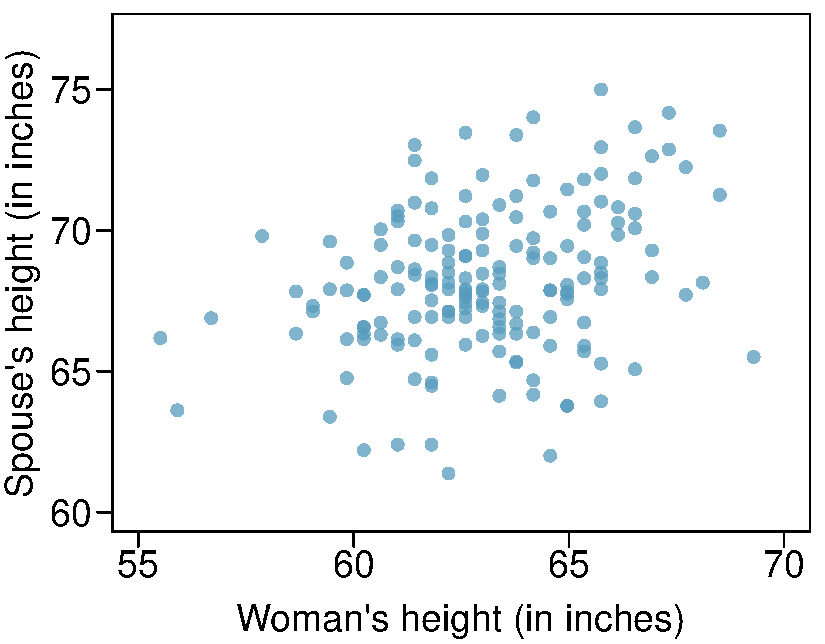
\includegraphics[width=\textwidth]{husbands_wives_height_inf_2s}
\end{center}
\end{minipage}
\begin{minipage}[c]{0.6\textwidth}
{\scriptsize
\begin{center}
\begin{tabular}{rrrrr}
    \hline
                    & Estimate  & Std. Error    & t value   & Pr($>$$|$t$|$) \\ 
    \hline
(Intercept)         & 43.5755   & 4.6842        & 9.30      & 0.0000 \\ 
height\_\hspace{0.3mm}man   & 0.2863    & 0.0686        & 4.17      & 0.0000 \\ 
    \hline
\end{tabular}
\end{center}
}
\end{minipage}
\begin{parts}
\item Is there strong evidence in this sample that taller women have taller spouses? 
State the hypotheses and include any information used to conduct the test.
\item Write the equation of the regression line for predicting the height of a woman's spouse based on the woman's height.
\item Interpret the slope and intercept in the context of the application.
\item Given that $R^2 = 0.09$, what is the correlation of heights 
in this data set?
\item You meet a married woman from Britain who is 5'9" (69 inches). 
What would you predict her spouse's height to be? How reliable is this 
prediction?
\item You meet another married woman from Britain who is 6'7" (79 inches). 
Would it be wise to use the same linear model to predict her spouse's 
height? Why or why not?
\end{parts}